\chapter{Non imaging optics}
This chapter provides the notions of illumination optics needed in this thesis. We start explaining the difference between radiometry and photometry.
In particular, we focus on the photometric variables defining them both in three and two dimensions. The reflection and refraction laws and the phenomenon of total internal reflection are explained. The last paragraph of the chapter gives a brief introduction of the Fresnel's equations. 
\section{Radiometric and photometric variables}
Radiometry is the measurement of the electromagnetic radiation across the entire electromagnetic spectrum. Photometry is the subfield of radiometry that takes into account only the portion of the electromagnetic spectrum corresponding to the visible light, \cite{zalewski1995radiometry}. Radiometry deals with radiometric quantities. An important radiometric quantity  is the radiant flux $\Phi_{\textrm{r}}$ (unit watt, [\textrm{W}]) which is the total energy emitted from a source or received by a target per unit time:
\begin{equation}
\Phi_{\textrm{r}} = \frac{\textrm{d}Q}{\textrm{d}T}\,,
\end{equation}
where $Q$ is the energy and $T$ the time.\\
\indent In Illumination optics the measurement of light is given in terms of the impression that it gives on the human eyes. Therefore, illumination optics deals with the photometric variables. The most important photometric variables are defined as in the following. The luminous flux $\Phi$ (unit lumen, [\textrm{lm}]) is defined as the perceived power of light by the human eye, \cite{chaves2015introduction}.
 The radiant and the luminous flux are related by the luminous efficacy function, unit [lm/W], that tells us how many lumen there are for each Watt of power at a given wavelength.
 The luminous efficacy reaches its maximum  at a wavelength of $555$ $\textrm{nm}$ where it is equal to $683$ $\textrm{lm}/\textrm{W}$.
  We may normalize the luminous efficacy function with its maximum value of $683$.
  This normalized function is the dimensionless luminosity function $\bar{y}(\lambda)$ shown in Figure $\ref{fig:luminosityfunction}$ where $\lambda$ is the wavelength.
\begin{figure}[h]
%\label{fig:luminousfunction}
  \begin{center}
  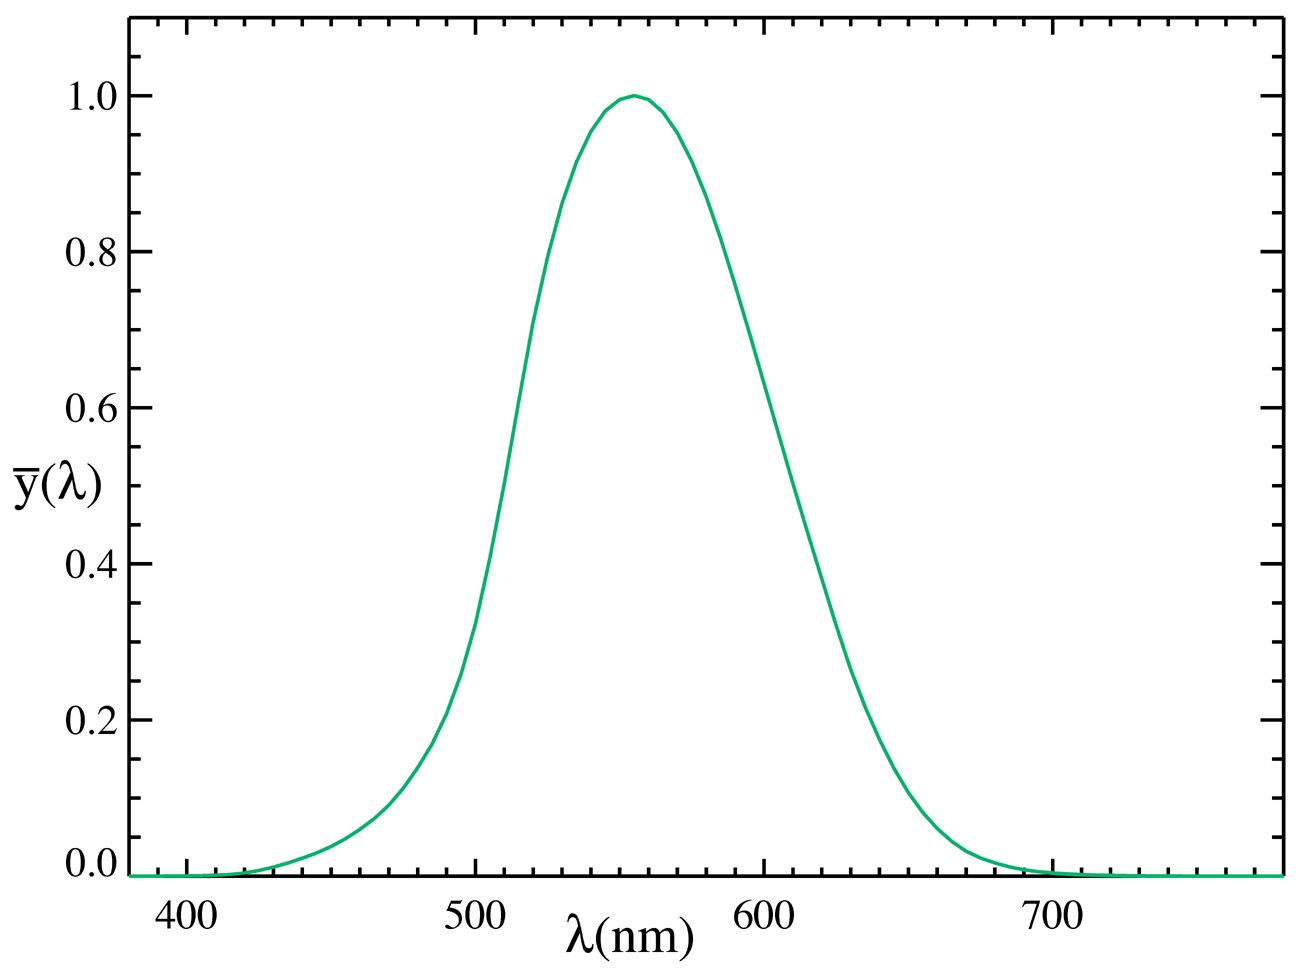
\includegraphics[width=7cm]{CIELuminosity}
  \end{center}
  \caption{Luminosity function $\bar{y}(\lambda)$: relation between the eye's sensitivity and the wavelength of the light. The luminous function is dimensionless.}
  \label{fig:luminosityfunction}
  \end{figure}
\\ The luminous flux corresponding to one Watt of radiation power at any wavelength is given by the product of $683$ $\textrm{lm/W}$ and the luminosity function at the same wavelength,
i.e. $683 \, \bar{y}(\lambda)$. Hence, $\Phi$ has unit lumen [\textrm{lm}] and it is defined as:
\begin{equation}
\Phi = 683 \int_0^\infty \Phi_\textrm{r}(\lambda) \bar{y}(\lambda)\textrm{d}\lambda \;.
\end{equation}
\indent The luminous flux $\textrm{d}\Phi$ falling on a surface is called illuminance $E$ \big(unit \big[$\textrm{lm}/\textrm{m}^2\big]$\big)
and is defined as:
\begin{equation}
 E=\frac{\textrm{d}\Phi}{\textrm{d}A}\;,
 \end{equation}
 where $\textrm{d}A$ is an infinitesimal area receiving energy. \\
\indent A beam of light can be described as a collection of light rays, where a light ray can be seen as a path along which the energy travels. The density of light emitted by a point source in a given direction is determined by the solid angle. The solid angle subtended by the light is defined by the infinitesimal surface area $\textrm{d}A^*$  of a sphere subtended by the radius of that sphere and by the rays emitted by the point source.  The solid angle is indicated with $\Omega$ and the dimensionless unit of solid angles is the steradian $[sr]$, \cite{arecchi2007field}. Indicating with $r$ the radius of the sphere, the infinitesimal solid angle $\textrm{d}\Omega$ defined by $\textrm{d}A^*$  is given by:
\begin{equation}\label{solid_angle}
\textrm{d}\Omega = \frac{\textrm{d}A^*}{r^2} 
\end{equation}
The luminous intensity $I$ (unit candela (\textrm{cd}), $[\textrm{cd}=\textrm{lm}/\textrm{sr}]$) is defined as the luminous flux $\textrm{d}\Phi$ per solid angle
$\textrm{d}\Omega$ and is given by:
\begin{equation}\label{intensity}
I = \frac{\textrm{d}\Phi}{\textrm{d}\Omega}\;.
\end{equation}
 \begin{figure}[h]
%\label{fig:cup}
  \begin{center}
  \includegraphics[width=6 cm]{solid_Angle}
  \end{center}
  \caption{Solid angle $\textrm{d}\Omega$ in a direction making an angle \myangle with the normal to the area $\textrm{d}A$.}
  \label{fig:rad}
  \end{figure}
The luminance $L$ \big(unit $\big[\textrm{cd} / \textrm{m}^2\big]$\big) is the luminous flux per unit solid angle $\textrm{d}\Omega$ and  per unit projected area $\cos(t)\,\textrm{d}A$ where $t$ is the angle that the normal $\boldsymbol{\nu}$ to area $\textrm{d}A$ makes with the direction of the solid angle $\textrm{d}\Omega$, as shown in Figure $\ref{fig:rad}$.  $L$  is given by:
\begin{equation}\label{luminance1}
  L=\frac{\textrm{d}\Phi}{\cos \mbox{\myangle}\textrm{d}A\textrm{d}\Omega}.
\end{equation}
\noindent Note that from ($\ref{intensity}$) and ($\ref{luminance1}$) we can derive a relation between the intensity and the luminance.\\
The infinitesimal intensity $\textrm{d}I $ emitted by the area element $\textrm{d}A$ is given by:
\begin{equation}
\textrm{d}I = \frac{\textrm{d}\Phi}{\textrm{d}\Omega}= L(\textrm{x},\mbox{\myangle})\cos(\mbox{\myangle})\textrm{d}A \,.
\end{equation}
When the luminance is uniform over a finite area $A$, the luminous intensity emitted in the direction \myangle is equal to:
\begin{equation}
I(t) = L(\mbox{\myangle}) A \cos(\mbox{\myangle})\,.
\end{equation}
Thus, when $L(\textrm{x},\mbox{\myangle})$ does not depend on the position and the direction (i.e. $L(\textrm{x},\mbox{\myangle})=L$), we deduce Lambert's cosine law:
\begin{equation}
I(t) = I_0\cos(\mbox{\myangle})\,.
\end{equation}
where $I_0 = I(0) = LA$. \\
Finally the \'{e}tendue $U$ (unit $[m \cdot srad]$) describes the ability of a source to emitt light or the capability of an optical system to receive light, \cite{zhu2011etendue}.
The quantity $ \textrm{d}U $ is defined as:
\begin{equation}\label{etendue}
\textrm{d}U = n^2 \cos(\mbox{\myangle}) \textrm{d}A\textrm{d}\Omega.
\end{equation}
where $n$ is the index of refraction of the medium in which the surface $A$ is immersed. In optics the \'{e}tendue is considered to be a volume in phase space  (or an area for two-dimensional systems). This concept will be clarified in Chapter \ref{chap:PS} where we treat the phase space in more details.
An important property of the \'{e}tendue is that it is conserved within an optical system where the flux is constant. We now show, following the same approach used by J. Chaves in \cite{chaves2015introduction}, how the conservation of this quantity can be derived .
Consider a light ray emitted from an infinitesimal area $\textrm{d}A_1$ to the area $\textrm{d}A_2$ located at a distance $d$ from $\textrm{d}A_1$,  see Figure \ref{fig:etendue_conservation}.
\begin{figure}[h]
 \label{fig:etendue_conservation}
     \begin{center}
     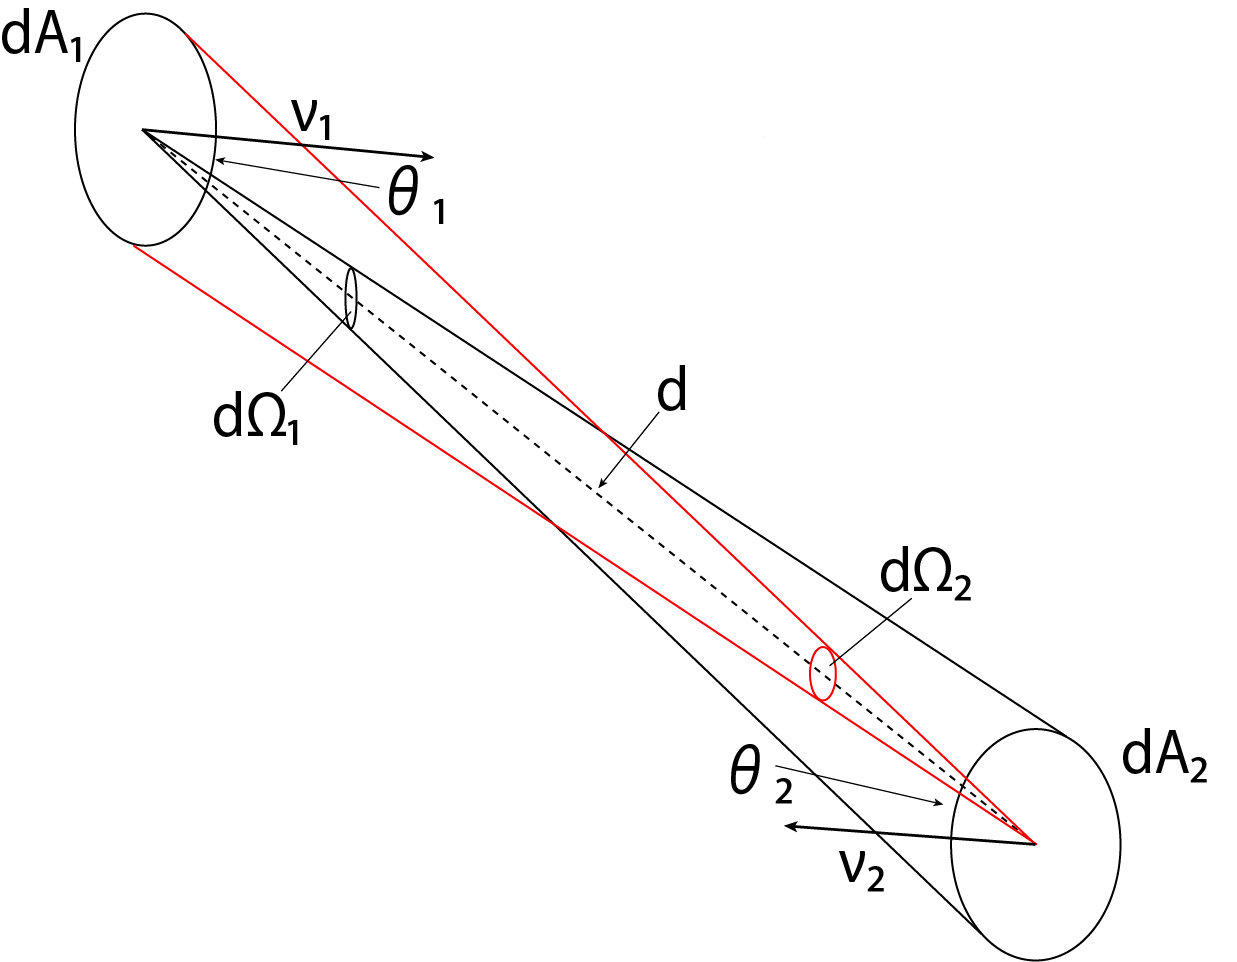
\includegraphics[width=10cm]{areas.png}
     \end{center}
     \caption{\footnotesize{$\textrm{d}A_1$ and $\textrm{d}A_2$ are two line surfaces with normal $\nu_1$ and $\nu_2$, respectively. \myangle$_1$ and \myangle$_2$ are the angles made by the central ray with the normals $\nu_1$ and $\nu_2$, respectively.}}
\label{fig:etendue_conservation}
 \end{figure}
\\ Indicating with $\boldsymbol{\nu}_1$ and $\boldsymbol{\nu}_2$ the normals to the surfaces $\textrm{d}A_1$ and $\textrm{d}A_2$, respectively and with \myangle$_1$ and \myangle$_2$ the angles that the central ray forms with $\boldsymbol{\nu}_1$ and $\boldsymbol{\nu}_2$, respectively,
the flux passing though $\textrm{d}A_2$ coming from $\textrm{d}A_1$ is defined as:
\begin{equation}
\textrm{d}\Phi_1 = L \cos(\mbox{\myangle}_1) \textrm{d}A_1 \textrm{d}\Omega_1
\end{equation}
where $\textrm{d}\Omega_1$ is defined at the area $\textrm{d}A_1$ by the area $\textrm{d}A_2$ and it is given by 
\begin{equation}
\textrm{d}\Omega_1 = \frac{\textrm{d}A_2\cos(\mbox{\myangle}_2)}{d^2}\,.
\end{equation}
Similarly, the flux passing though $\textrm{d}A_1$ coming from $\textrm{d}A_2$ is equal to:
\begin{equation}
\textrm{d}\Phi_2 = L \cos(\mbox{\myangle}_2) \textrm{d}A_2 \textrm{d}\Omega_2
\end{equation}
and
\begin{equation}
\textrm{d}\Omega_2 = \frac{\textrm{d}A_1\cos(\mbox{\myangle}_1)}{d^2}\,.
\end{equation}
Then \begin{equation}
\label{etendue1}
\textrm{d}U_1 = n^2 \textrm{d}A_1\cos(\mbox{\myangle}_1)\textrm{d}\Omega_1= \frac{n^2 \textrm{d}A_1\cos(\mbox{\myangle}_1)\textrm{d}A_2\cos(\mbox{\myangle}_2)}{d^2},
\end{equation}
and
\begin{equation}
\label{etendue2}
\textrm{d}U_2 = n^2 \textrm{d}A_2\cos(\mbox{\myangle}_2)\textrm{d}\mbox{\myangle}_2= \frac{ n^2 \textrm{d}A_2\cos(\mbox{\myangle}_2)\textrm{d}A_1\cos(\mbox{\myangle}_2)}{d^2}\,.
\end{equation}
From equation ($\ref{etendue1}$) and ($\ref{etendue2}$) we see that $\textrm{d}U_1=\textrm{d}U_2$.
For a light beam, all the light passing through $\textrm{d}A_1$ coincides with the light passing through $\textrm{d}A_2$, hence $\textrm{d}U = \textrm{d}U_1$. Moreover, for the same light beam, all the light passing from $\textrm{d}A_2$ corresponds to the light emitted from $\textrm{d}A_1$, then $\textrm{d}U=\textrm{d}U_2$. Finally we can conclude that the \'{e}tendue $\textrm{d}U$ is conserved along a beam of light. Since also the flux through the areas $\textrm{d}A_1$ and $\textrm{d}A_2$ is conserved, the following relation holds:
\begin{equation}\label{basicluminance}
L := n \frac{\textrm{d}\Phi}{\textrm{d}U} = constant\,.
\end{equation}
 In the optical systems we will consider in this work, the source and the target are located in the same medium (air) with $n=1$, so the luminance $L$ equals the basic luminance $L^* = L/n$ at the source and the target of the system.\\
\indent In this thesis we consider two-dimensional optical systems. 
 Hence, we need to find two-dimensional analogies for the definitions given above.
In two dimensions the illuminance \big(unit $\big[\textrm{lm}/\textrm{m}\big]$\big) denotes the luminous flux falling on an infinitesimal line segment of length $\textrm{d}x$ and it is given by:
 \begin{equation}
 E=\frac{\textrm{d}\Phi}{\textrm{d}x}\;.
 \end{equation}
 The luminous intensity \big(unit $\big[\textrm{lm}/\textrm{rad}\big]$\big) is the luminous flux per angle $\textrm{d}t$:
 \begin{equation}
 I=\frac{\textrm{d}\Phi}{\textrm{d}\mbox{\myangle}}\;.
 \end{equation}
 Thus the following relation holds:
 \begin{equation}
 \textrm{d}I = L\cos(t)\textrm{d}x\,.
 \end{equation}
 The $2D$ luminance \big(unit $\big[\textrm{lm}/(\textrm{rad}\; \textrm{m})\big]$\big) is given by:
 \begin{equation}
 L = \frac{\textrm {d}\Phi}{\cos t\,\textrm{d}x \,\textrm{d}\mbox{\myangle}}.
 \end{equation}
  The \'{e}tendue $\textrm{d}U $ (unit $[m\cdot rad]$) in $2$D is given by:
\begin{equation}\label{etendue2d}
\textrm{d}U = n\cos(\mbox{\myangle}) \textrm{d}a\textrm{d}\mbox{\myangle}.
\end{equation}



\section{Reflection and refraction law}
The propagation of a light ray traveling through  different media is described by the reflection and refraction law.
In this section we introduce these two laws and we explain the total internal reflection phenomenon.
A light ray is described by a position vector \vect{x} and a direction vector \vect{t} and can be parameterized by the arc length \variabile{s}.
Light rays travel in an homogeneous medium along straight lines, once they hit a reflective surface their direction changes.
 Denoting with $\vect{t}_i$ the direction of the incident ray and with $\boldsymbol{\nu}$ the unit normal to the surface at the location of the incidence, the direction $\vect{t}_r$ of the reflected ray is given by:
 \begin{equation}\label{Reflection}
  \vect{t}_r = \vect{t}_i-2(\vect{t}_i,\boldsymbol{\nu})\boldsymbol{\nu}\,,
\end{equation}
where the vectors $\vect{t}_i$ and $\boldsymbol{\nu}$ are unit vectors. 
From Eq. (\ref{Reflection}) it follows that the vector  $\vect{t}_r$ is a unit vector too, indeed considering the scalar product $(\vect{t}_r,\vect{t}_i)$ it holds:
\begin{equation}\label{unit_vector}
(\vect{t}_r,\vect{t}_i) = (\vect{t}_r,\vect{t}_i) - 4(\vect{t}_r,\boldsymbol{\nu})(\vect{t}_i,\boldsymbol{\nu})+
4(\vect{t}_i,\boldsymbol{\nu})^2(\boldsymbol{\nu},\boldsymbol{\nu})=1 .
\end{equation} 
Denoting the incident angle with \myangle$_i$ and the reflective angle with \myangle$_r$ such that
\begin{equation}
\cos{\mbox{\myangle}_i} = -\vect{t}_i\cdot \boldsymbol{\nu} \qquad \mbox{and} \qquad \cos{\mbox{\myangle}_r} = \vect{t}_r \cdot\boldsymbol{\nu}\,,
\end{equation}
the reflection law states that \myangle$_i$ equals \myangle$_r$ which are measured counterclockwise with respect to the normal $\boldsymbol{\nu}$ of the surface, see Fig. \ref{fig:Snell}.
\begin{figure}[h]
 \label{fig:Snell}
     \begin{center}
     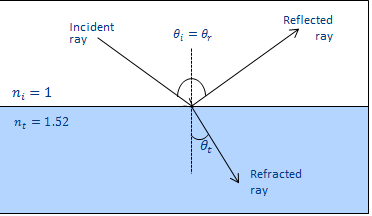
\includegraphics[width=8cm]{Snell.png}
     \end{center}
     \caption{\footnotesize{$\textrm{d}A_1$ and $\textrm{d}A_2$ are two line surfaces with normal $\nu_1$ and $\nu_2$, respectively. $t_i$ and $t_2$ are the angles made by the central ray with the normals $\nu_1$ and $\nu_2$, respectively.}}
\label{fig:Snell}
 \end{figure}
\\ When a ray propagates through two media with two different media, it direction changes according to refraction law. 
Indicating with $n_i$ the index of refraction of the medium in which the incident ray travels and with $n_t$ the index of refraction of the medium of the transmitted ray, the direction $\vect{t}_t$ of the transmitted ray is given by:
\begin{equation}\label{Refraction}
\vect{t}_t = n_{i,t}\,\vect{t}_i+
\Big[\sqrt{1-n_{i,t}^2+n_{i,t}^2(\boldsymbol{\nu},\vect{t}_i)^2}-n_{i,t}(\boldsymbol{\nu},\vect{t}_i) \Big]\boldsymbol{\nu}\,,
\end{equation}
where $n_{i,t}=n_i/n_t$. \\
 \indent Note that in Eq. (\ref{Reflection}) the direction of the normal $\boldsymbol{\nu}$ to the surface is not relevant for the computation of the direction of the reflective ray, since:
\begin{equation}
\vect{t}_r = \vect{t}_i-2(\vect{t}_i,\boldsymbol{\nu})\boldsymbol{\nu}= \vect{t}_i-2(\vect{t}_i,-\boldsymbol{\nu})(-\boldsymbol{\nu}) ,
\end{equation}
while this is not the case of Eq. (\ref{Refraction}), therefore in the latter case we need to specify the direction of $\boldsymbol{\nu}$ which is usually chosen in such a way that the angle that it forms with the incident ray $\vect{t}_i$ is smaller than or equal to $\pi/2$. Hence, if $(\vect{t}_i, \boldsymbol{\nu})\geq0$ the normal $\boldsymbol{\nu}$ directed inside the same medium in which travels the incident ray is taken, otherwise the normal $-\boldsymbol{\nu}$ directed inside the same medium in which the transmitted ray will travel has to be considered. \\ \indent
Eq. (\ref{Refraction}) is only valid for 
\begin{equation}\label{tir}\begin{split}
1-n_{i,t}^2+n_{i,t}^2(\boldsymbol{\nu},\vect{t}_i)^2\geq 0 & \Rightarrow \frac{n_t}{n_i}\geq \sqrt{1-(\boldsymbol{\nu},\vect{t}_i)^2}\\
\Rightarrow n_t\geq n_i\sqrt{1-\cos^2(\mbox{\myangle}_i)} & \Rightarrow  n_t\geq n_i \sin(\mbox{\myangle}_i)
\end{split}
\end{equation}
 The angle for which the equality holds is
\begin{equation}\label{critical}
\mbox{\myangle}_{\textrm{c}} = \arcsin\Big(\frac{n_t}{n_i}\Big)
\end{equation} and it is called the critical angle, \cite{chaves2015introduction}.
Note that the condition $\frac{n_t}{n_i}<1$ is verified as in this case $\sin(\mbox{\myangle}_\textrm{i})<1$.
When the incident angle \myangle$_{\textrm{i}}$ is exactly equal to the critical angle \myangle$_{\textrm{c}}$ the refractive ray propagates parallel to the refractive surface, 
when \myangle$_{\textrm{i}}>\mbox{\myangle}_{\textrm{c}}$ the light ray is no longer refracted but it is reflected by the surface. This phenomenon is called total internal reflection (TIR). When TIR occurs, the $100\%$ of light is reflected and there is no loss of energy. Therefore, optical systems designed such that TIR is always verified are very efficient. In general, light that hits a normal refractive mirror can be both reflected and refracted. Therefore, some part of the energy is transmitted and some part is reflected. The amount of light that is reflected and refracted is determined by the Fresnel's coefficients.
In the next paragraph an overview of  Fresnel equations is given.

\section{The Fresnel equations}
In order to derive Fresnel's equations we need to describe light as an electromagnetic wave. 
It is therefore useful to study the light propagation from the perspective of Electromagnetic Theory which gives information about the incident, reflected and transmitted radiant flux density that are denoted with $E_i$, $E_r$ and $E_t$, respectively.  
Any component of the electric field $\boldsymbol{\mathcal{E}}$ can be written in the form
\begin{equation}
\boldsymbol{\mathcal{E}}(\vect{x}, \mytime) = \boldsymbol{\mathcal{E}}_0(\vect{x} )e^{i(\omega \mytime - \vect{k}\cdot \vect{r})}
\end{equation}
where the amplitude $\boldsymbol{\mathcal{E}}_0(\vect{x})$ is constant in time. The vector \vect{k} has the same direction of the wave and its absolute value 
$|\vect{k}| = k = \frac{2\pi}{\lambda}$ is the wave number in vacuum, with $\lambda$ the wavelength. The value of the angular frequency is $\omega = \frac{c k}{n}$ with $c$ the velocity of the light and $n$ the index of refraction in which the wave is traveling that is the ratio of the speed of light $v$ in the material and the speed of light $c$ in vacuum.
Similarly, the magnetic field has the form:
\begin{equation}
\boldsymbol{\mathcal{B}}(\vect{x}, \mytime) = \boldsymbol{\mathcal{B}}_0(\vect{x}) e^{i(\omega \mytime - \vect{k}\cdot \vect{r})}\,.
\end{equation}
In the field of electromagnetism a very important concept is the Poynting vector \vect{P}. 
It defines the energy flux of an electromagnetic field,  it is measured in $[W/m^2]$ and it is defined as:
\begin{equation}
\vect{P} = \frac{1}{\mu}\Big(\mathcal{E}\times \mathcal{B}\Big)
\end{equation}
where $\mu = \frac{1}{\varepsilon v^2}$ is the permeability and $\varepsilon$ the permittivity. In the following, the vacuum parameters are indicated with the subscript $0$. All the quantities defined in the media of the incident, reflective and transmitted light are indicated with the subscripts $i$, $r$ and $t$, respectively. Optical rays are perpendicular to the wave front of an electromagnetic wave and parallel to the Poynting vector, \cite{jones2015optical}.
The irradiance $E$ is defined as the average energy that crosses in unit time a unit area $A$ perpedicular to the direction of the energy flow.
Therefore:
\begin{equation}
\vect{E} = <\vect{P}>_{\mytime} = \frac{c}{2\mu_0}\boldsymbol{\mathcal{E}}_0^2\,,
\end{equation}
where $<\cdot>_\mytime$ indicates the average in time.
Considering a beam of light that hit a surface such that an area $A$ is illuminated, the incident, reflected and transmitted beams are $\vect{E}_i A\cos(\mbox{\myangle}_i)$ $\vect{E}_r A\cos(\mbox{\myangle}_r)$ and $\vect{E}_t A\cos(\mbox{\myangle}_t)$ , respectively.
The reflectance $\mathcal{R}$ is the ratio of the reflected power to the incident power:
\begin{equation}\label{reflectance}
\mathcal{R} = \frac{\vect{E}_r A\cos(\mbox{\myangle}_r)}{\vect{E}_i A\cos(\mbox{\myangle}_i)} 
\end{equation}
Similarly, the transmittance $T$ is the ratio between the transmitted to the incident power:
\begin{equation}\label{transmittance}
\mathcal{T} = \frac{\vect{E}_tA\cos(\mbox{\myangle}_t)}{\vect{E}_r A\cos(\mbox{\myangle}_r)}
\end{equation}\\
Note that, since  $\vect{E} _r/\vect{E}_t = (v_r\varepsilon_r \boldsymbol{\mathcal{E}}_{0r}^2/2)/(v_i\varepsilon_i \boldsymbol{\mathcal{E}}_{0i}^2/2)$, Eq. (\ref{reflectance}) becomes
\begin{equation}\label{R}
\mathcal{R} = \Bigg(\frac{\boldsymbol{\mathcal{E}}_{0 r}}{\boldsymbol{\mathcal{E}}_{0 i}}\Bigg)^2\,,
\end{equation} 
while Eq. (\ref{transmittance}) gives: \begin{equation}\label{T}
\mathcal{T} = \frac{n_t \cos(\mbox{\myangle}_t)}{n_t \cos(\mbox{\myangle}_i)}\Bigg(\frac{\boldsymbol{\mathcal{E}}_{0 t}}{\boldsymbol{\mathcal{E}}_{0 i}}\Bigg)^2
\end{equation}
where we assumed that $\mu_i = \mu_t  = \mu_0$ and we used the fact that $\mu_0 v_t\varepsilon_t=n_t/c$.
Employing the total energy conservation, that is:
\begin{equation}
\vect{E}_i A\cos(\mbox{\myangle}_i) = \vect{E}_r A\cos(\mbox{\myangle}_r)+\vect{E}_t A\cos(\mbox{\myangle}_t)\,,
\end{equation}
it can be easily proved that:
\begin{equation}
\mathcal{R}+\mathcal{T}=1\,.
\end{equation}
The values $r = \Big(\frac{\boldsymbol{\mathcal{E}}_{0 i}}{\boldsymbol{\mathcal{E}}_{0 i}}\Big)$ and 
$t = \Big(\frac{\boldsymbol{\mathcal{E}}_{0 t}}{\boldsymbol{\mathcal{E}}_{0 i}}\Big)$ are called the amplitude coefficients.  
The intensity of the reflected and transmitted light depends not only on the angle of incidence but also on the polarization of the electromagnetic field.
By convention, we refer to the polarization of electromagnetic waves as the direction of the electric field $\boldsymbol{\mathcal{E}}$, 
\cite{feynman1964feynman}. When $\boldsymbol{\mathcal{E}}$ is perpendicular to the plane of incidence, light is called $s$-polarized, while when
$\boldsymbol{\mathcal{E}}$ is parallel to the plane of incidence, it is said that light is $p$-polarized.
For $s$-polarized light the perpendicular components $r_s$ and $t_s$ of $r$ and $t$ are defined. 
For $p$-polarized light the parallel components $r_p$ and $t_p$ of $r$ and $t$ are given. 
Those coefficients are obtained considering the Maxwell's equations and the boundaries conditions due to the conservation of energy.
For the first case ($s$-polarization), the boundaries conditions are given by the conservation of the tangent component of $\boldsymbol{\mathcal{E}}$ and of the normal component of $\boldsymbol{\mathcal{B}}$. For the second case ($p$-polarization), the boundaries conditions are given by the conservation of the tangential component $\boldsymbol{\mathcal{E}}$ and of the tangent component of $\boldsymbol{\mathcal{B}}$. These conditions together with Maxwell's equations lead to four equations with four unknowns.
Solving those equations the Fresnel coefficients are derived. 
It is out of this work to show the details of Fresnel equations as they are widely explained in the leterature. 
In the following we provide Fresnel coefficients and we briefly explain their physical interpretation. We refer the reader to \cite{born2013principles, hecht1998hecht} for more details. 
Fresnel's coefficients can also be derived using a different approach that does not involves Marxwell's equations, this method is widely explained in \cite{feynman2011feynman}. 
In case \vect{E} is perpendicular to the plane of incidence the following results are obtained:
\begin{equation} \label{Fresnel_perpendicular}
\begin{split}
r_{s} & = \frac{n_i\cos(\mbox{\myangle}_i)-n_t \cos(\mbox{\myangle}_t)}{n_i \cos(\mbox{\myangle}_i)+n_t\cos(\mbox{\myangle}_t)}\\
t_{s} & =  \frac{2n_i\cos(\mbox{\myangle}_i)}{n_i\cos(\mbox{\myangle}_i)+n_t\cos(\mbox{\myangle}_t)}
\end{split}
\end{equation}
In case \vect{E} is parallel to the plane of incidence the amplitude coefficients are:
\begin{equation}\label{Fresnel_parallel}
\begin{split}
r_{p} & = \frac{n_t\cos(\mbox{\myangle}_i)-n_i \cos(\mbox{\myangle}_t)}{n_i \cos(\mbox{\myangle}_t)+n_t\cos(\mbox{\myangle}_i)}\\
t_{p} & =  \frac{2n_i\cos(\mbox{\myangle}_i)}{n_i\cos(\mbox{\myangle}_t)+n_t\cos(\mbox{\myangle}_i)}.
\end{split}
\end{equation}
Using Snell's Law, Equations (\ref{Fresnel_perpendicular}) and (\ref{Fresnel_parallel}) are simplified as in the following:
\begin{equation} \label{simple_Fresnel}
\begin{split}
r_{s} & = -\frac{\sin(\mbox{\myangle}_i-\mbox{\myangle}_t)}{\sin(\mbox{\myangle}_i+\mbox{\myangle}_t)}\\
r_{p} & =  +\frac{\tan(\mbox{\myangle}_i-\mbox{\myangle}_t)}{\mbox{\myangle}_i+\mbox{\myangle}_t}\\
t_{s} & = -\frac{2\sin \mbox{\myangle}_t \cos \mbox{\myangle}_i}{\sin(\mbox{\myangle}_i+\mbox{\myangle}_t)}\\
t_{p} & = +\frac{2\sin \mbox{\myangle}_t \cos \mbox{\myangle}_i}{\sin(\mbox{\myangle}_i+\mbox{\myangle}_t)\cos(\mbox{\myangle}_i- \mbox{\myangle}_t)}.
\end{split}
\end{equation}
It can be show that
 \begin{equation}
\begin{split}
t_s+(-r_s) &= 1 \\
t_p+r_p &=  1
\end{split}
\end{equation}
Fresnel coefficients are shown in Fig. \ref{fig:coefficients} for the case in which light travels from a less dense to a more dense medium ($n_i<n_t$), that is external reflection. 
While in Fig. \ref{fig:coefficients2} the coefficients are shown for the case in which $n_i>n_t$, that is internal reflection. Note from Fig. \ref{fig:coefficients} that $r_p$ approaches to $0$ when \myangle$_i$ approaches to \myangle$_p$ and it gradually decreases reaching $-1$ for an incident angle \myangle$_i=90^\circ$. The angle \myangle$_p$ is called Brewster's angle or polarization angle as only the component perpendicular to the incident ray will be reflected and therefore light is perfectly polarized. Similarly, Fig. \ref{fig:coefficients2} shows that $r_p=0$ for \myangle$_i=$\myangle$_{p\prime}$. It can be show that \myangle$_p+$\myangle$_{p\prime}= 90^\circ$. Fig. \ref{fig:coefficients2} also shows that $r_p$ and $r_s$ reach $1$ when \myangle$_i=$\myangle$_c$. \myangle$_c$ is called the critical angle. Light that hits the incident plane with an incident angle equal to or greater than the critical angle is totally reflected back and no transmitted light is observed. This phenomenon is called total internal reflection. 
\begin{figure}[h]
  \begin{minipage}[h]{0.4\textwidth}
    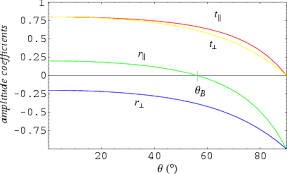
\includegraphics[width=\textwidth]{amplitude_coefficients2.png}
    \caption{Amplitude coefficients of reflection and transmission as a function of the incident angle \myangle$_i$ in the case of external reflection, i.e. $n_t<n_i$. 
($n_t = 1$ and $n_i=1.5$).}
    \label{fig:coefficients}
  \end{minipage} \hspace{2.5cm}
  \begin{minipage}[h]{0.4\textwidth}
    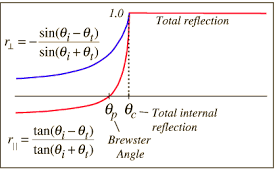
\includegraphics[width=\textwidth]{rprs.png}
    \caption{Amplitude coefficients of reflection as a function of the incident angle \myangle$_i$ in the case of internal reflection, i.e. $n_t>n_i$. 
($n_t = 1.5$ and $n_i=1$).}
   \label{fig:coefficients2}
 \end{minipage}
\end{figure}
\\ The parallel and perpendicular components of $\mathcal{R}$ and $\mathcal{T}$ are:
\begin{equation}\label{Fresnel_pands}
\begin{split}
\mathcal{R}_p& =  {r_p^2}\\
\mathcal{T}_p &=  \frac{n_t \cos(\mbox{\myangle}_t)}{n_t \cos(\mbox{\myangle}_i)}t_p^2\\
\mathcal{R}_s &=  r_s^2\\
\mathcal{T}_s &= \frac{n_t \cos(\mbox{\myangle}_t)}{n_t \cos(\mbox{\myangle}_i)}t_s^2\\
\end{split}
\end{equation}
it can be show that
\begin{equation}
\begin{split}
\mathcal{R}_s+\mathcal{R}_p &= 1\\
\mathcal{T}_s+\mathcal{T}_p &=1\,.
\end{split}
\end{equation}
For normal incidence, i.e. \myangle$_i = 0$, there is no polarization and Eqs. (\ref{Fresnel_pands}) lead to:
\begin{equation}
\mathcal{R} = \mathcal{R}_p = \mathcal{R}_s = \Bigg(\frac{n_i-n_t}{n_t+n_i}\Bigg)^2
\end{equation}
and 
\begin{equation}
\mathcal{T} = \mathcal{T}_p = \mathcal{T}_s = \frac{4n_i n_t}{(n_t+n_i)^2}\,.
\end{equation}
The behavior of the reflectance and transmittance is shown in Fig. \ref{fig:reflectance_and_transmittance}
\begin{figure}[t]
 \label{fig:Reflectance_transmittance}
     \begin{center}
     \includegraphics[width=10cm]{RandT.png}
     \end{center}
     \caption{\footnotesize{Top: Transmittance as a function of the incident angle both for the case of external reflection (top left) and internal reflection (top right).\\
Bottom: Reflectance as a function of the incident angle both for the case of external reflection (bottom left) and internal reflection (bottom right).}}
\label{fig:reflectance_and_transmittance}
 \end{figure}






























































